%%%%%%%%%%%%%%%%%%%%%%%%%%%%%%%%%%%%%%%%%%%%%%%%%%%%%%%%%%%%%%%
%
% Welcome to Overleaf --- just edit your LaTeX on the left,
% and we'll compile it for you on the right. If you open the
% 'Share' menu, you can invite other users to edit at the same
% time. See www.overleaf.com/learn for more info. Enjoy!
%
%%%%%%%%%%%%%%%%%%%%%%%%%%%%%%%%%%%%%%%%%%%%%%%%%%%%%%%%%%%%%%%

% Inbuilt themes in beamer
\documentclass{beamer}

%packages:
% \usepackage{tfrupee}
% \usepackage{amsmath}
% \usepackage{amssymb}
% \usepackage{gensymb}
% \usepackage{txfonts}

% \def\inputGnumericTable{}

% \usepackage[latin1]{inputenc}                                 
% \usepackage{color}                                            
% \usepackage{array}                                            
% \usepackage{longtable}                                        
% \usepackage{calc}                                             
% \usepackage{multirow}                                         
% \usepackage{hhline}                                           
% \usepackage{ifthen}
% \usepackage{caption} 
% \captionsetup[table]{skip=3pt}  
% \providecommand{\pr}[1]{\ensuremath{\Pr\left(#1\right)}}
% \providecommand{\cbrak}[1]{\ensuremath{\left\{#1\right\}}}
% %\renewcommand{\thefigure}{\arabic{table}}
% \renewcommand{\thetable}{\arabic{table}}      

\setbeamertemplate{caption}[numbered]{}

\usepackage{enumitem}
\usepackage{tfrupee}
\usepackage{amsmath}
\usepackage{amssymb}
\usepackage{gensymb}
\usepackage{graphicx}
\usepackage{txfonts}

\def\inputGnumericTable{}

\usepackage[latin1]{inputenc}                                 
\usepackage{color}                                            
\usepackage{array}                                            
\usepackage{longtable}                                        
\usepackage{calc}                                             
\usepackage{multirow}                                         
\usepackage{hhline}                                           
\usepackage{ifthen}
\usepackage{caption} 
\captionsetup[table]{skip=3pt}  
\providecommand{\pr}[1]{\ensuremath{\Pr\left(#1\right)}}
\providecommand{\cbrak}[1]{\ensuremath{\left\{#1\right\}}}
\renewcommand{\thefigure}{\arabic{table}}
\renewcommand{\thetable}{\arabic{table}}   
\providecommand{\brak}[1]{\ensuremath{\left(#1\right)}}

% Theme choice:
\usetheme{CambridgeUS}

% Title page details: 
\title{Assignment 4} 
\author{Suryaansh Jain}
\date{\today}
\logo{\large \LaTeX{}}


\begin{document}

% Title page frame
\begin{frame}
    \titlepage 
\end{frame}

% Remove logo from the next slides
\logo{}


% Outline frame
\begin{frame}{Outline}
    \tableofcontents
\end{frame}



\section{Problem Statement}
\begin{frame}{Problem Statement}
    \begin{block}{13.5 Q12 [NCERT 12] } Find the probability of throwing at most 2 sixes in 6 throws of a single die.

    \end{block}
\end{frame}



\section{Definitions}
\begin{frame}{Random Variable Definition}
In this experiment, there are six consecutive Bernoulli trials. Let us define a Binomial Random Variable $X = \{0,1,2,3,4,5,6\}$ where the value of $X$ is the number of sixes obtained
  
\end{frame}



\begin{frame}{Probability Mass Function}

The probability of success (assuming a fair die) is $p=\frac{1}{6}$.

Therefore, the probability that $X$ maps to $i$ is given by:
\begin{block}{}
       \begin{align}
                \label{eq1}
           \pr{X=i} = \binom{6}{i} (1-p)^{6-i} p^i ,~ 0 \le i \le 6 
       \end{align}
\end{block}

The values for $i$ can be substituted in the above formula, and the graph of the PMF can be obtained.
\end{frame}


\begin{frame}{Cumulative Distribution Function}
The cumulative probability $ \pr{X \leq i}$ can be defined as under:

\begin{block}{}
\begin{align}
          \label{eq2}
       \pr{X \leq i} = \sum_{k=0}^{i} \binom{6}{k} (1-p)^{6-k} p^k ,~ 0 \le i \le 6
\end{align}
\end{block}

The values of $i$ can be substituted in the above equation, and the obtained values can be used to plot the CDF graph.

\end{frame}


\section{Solution}
\begin{frame}{Solution}

The probability to be found corresponds to the case $\pr{X \leq 2}$. Substituting $i$ in Equation \ref{eq1} and summing, we get
\begin{equation}
    \pr{X=2} + \pr{X=1} + \pr{X=0} = \frac{5^4}{3^3 \times 2^6} \approx 0.36
\end{equation}
\end{frame}

\section{Graphs}
\begin{frame}{PMF Graph}
The PMF graph is:
    \begin{figure}[!ht]
		\centering
		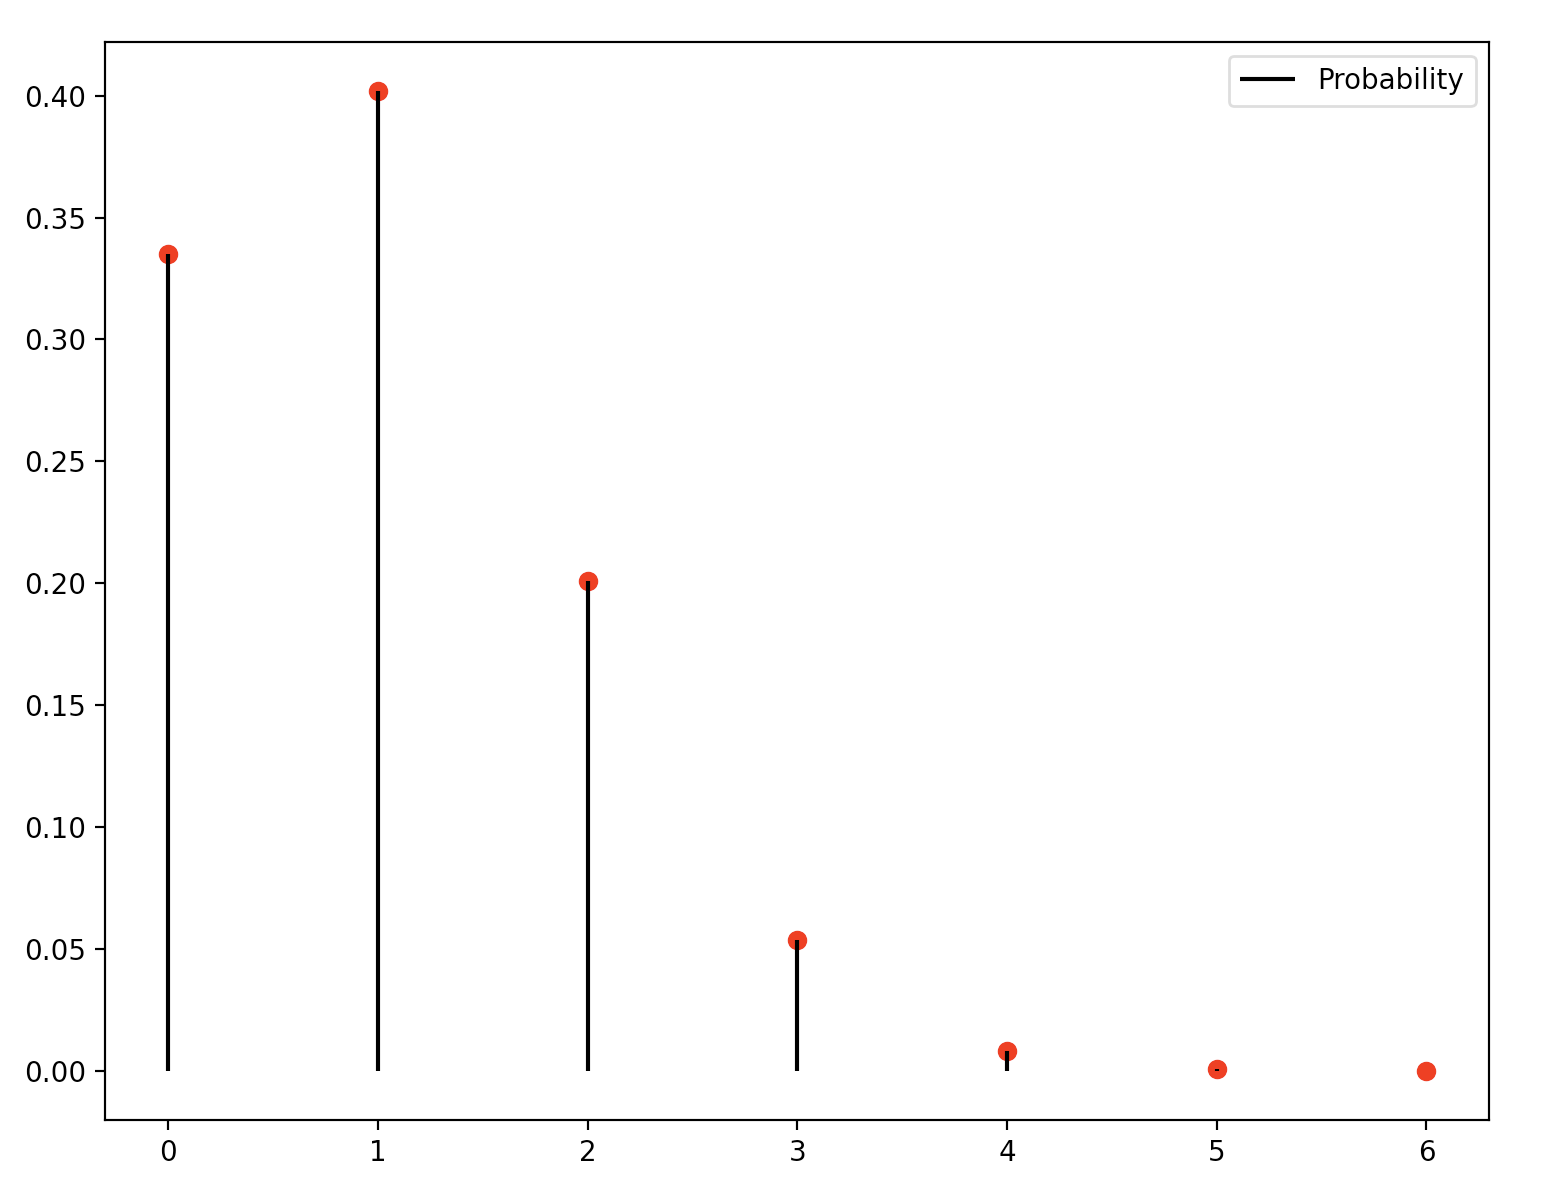
\includegraphics[width=\textwidth,height=5.5cm,keepaspectratio]{PMF.png}
		\label{fig1}
		\caption{Probability Mass Function}
	\end{figure}
\end{frame}

\begin{frame}{CDF Graph}
The CDF graph is:
    \begin{figure}[!ht]
		\centering
		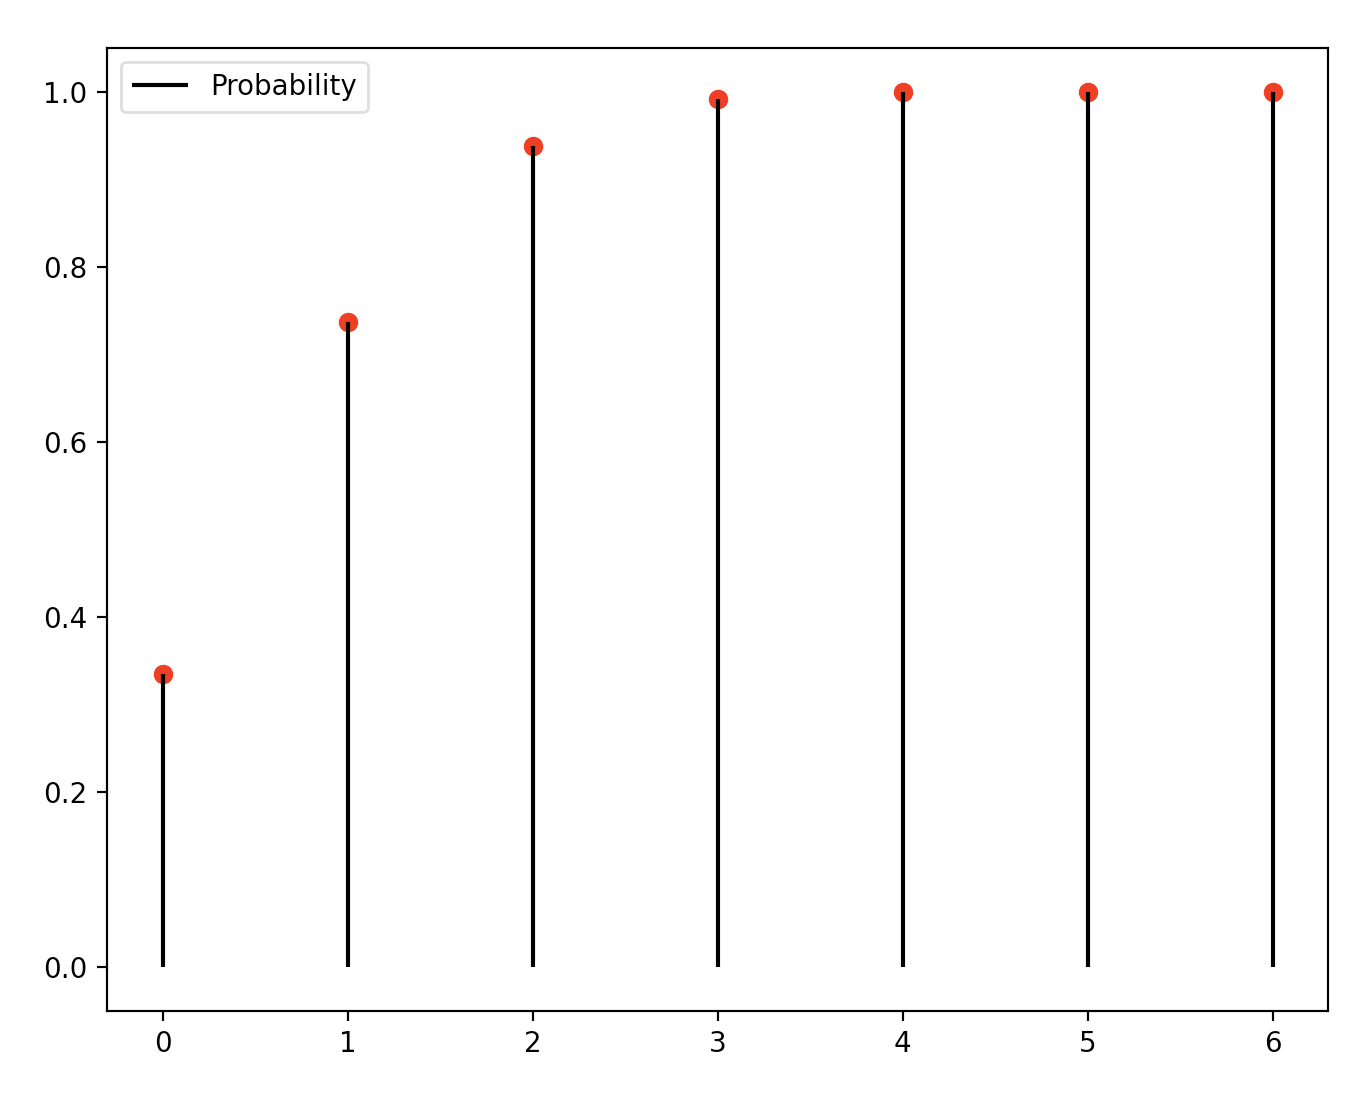
\includegraphics[width=\textwidth,height=5.5cm,keepaspectratio]{CDF.png}
		\label{fig2}
		\caption{Cumulative Distribution Function}
	\end{figure}
\end{frame}


\end{document}
